
\usepackage{fancyhdr}
\usepackage{lastpage}
\usepackage[utf8]{inputenc}

% Minted for syntax highliting
\usepackage{minted}
\usemintedstyle{tango}

% 
\usepackage[T1]{fontenc}
\usepackage{lmodern}

\usepackage{calc}
\usepackage{bytefield}

\usepackage{listings}
\usepackage{amsmath}

\usepackage{tikz}
\usetikzlibrary{automata,arrows,topaths,calc,positioning}
 
\usepackage{syntax}
\grammarindent=2cm


% Headers/footers styling
\pagestyle{fancy}
\fancyhf{}
\renewcommand{\headrulewidth}{0pt}

% Footer
\lfoot{ID1019}
\cfoot{KTH}
\rfoot{\thepage \hspace{1pt} / \pageref{LastPage}}

%\newcommand{\defaultpagestyle}{\thispagestyle{plain}}
\newcommand{\defaultpagestyle}{\thispagestyle{fancy}}




\title[ID1019 Introduction]{Introduction}

\author{Johan Montelius}
\institute{KTH}
\date{\semester}

\begin{document}

\begin{frame}
\titlepage
\end{frame}

\begin{frame}{introduction}
  Functional programming - what?
\end{frame}

\begin{frame}{variables, literals and builtin operations}

\begin{columns}[t]
 \begin{column}{0.4\linewidth}
   \begin{itemize}
     \pause \item {variables:} {\tt x}, {\tt y}, {\tt foo}, ..
     \pause \item {integer:} {\tt 1}, {\tt 23}, ..
     \pause \item {float:} {\tt 1.0}, {\tt 23.45}, ..
     \pause \item {bool:} {\tt true}, {\tt false} 
   \end{itemize}
 \end{column}
 \begin{column}{0.6\linewidth}
  \begin{itemize}
    \pause \item {binary operations:} {\tt +},{\tt -},{\tt *},{\tt /}, ..
    \pause \item {arithmetic functions:} {\tt div/2}, {\tt rem/2}, {\tt abs/1}, ..   
    \pause \item {comparison:} {\tt ==}, {\tt !=}, ..
    \pause \item {boolean operators:} {\tt and}, {\tt or}, ..
  \end{itemize}
 \end{column}
\end{columns}

\vspace{20pt}{\em There are more but this is fine for now.}

\vspace{20pt}{\em The notation {\tt div/2} means a function of two arguments.}


\end{frame}


\begin{frame}{functions}

  \begin{columns}[t]
    \begin{column}{0.5\textwidth}
  \begin{itemize}
   \pause \item {\tt fn x -> x + 2 end}
   \pause \item {\tt (fn x -> x + 2 end).(5)}
   \pause \item {\tt (5 + 2)}
   \pause \item {\tt 7}
  \end{itemize}
\end{column} \pause
\begin{column}{0.5\textwidth}
  \begin{itemize}
   \pause \item {\tt add = fn(x,y) -> x + y end}
   \pause \item {\tt add.(5, 4)}
   \pause \item {\tt (5 + 4)}
   \pause \item {\tt 9}
 \end{itemize}
\end{column}
\end{columns}\pause

\vspace{20pt}{\em Parenthesis are optional ... but quite nice to have.}

\vspace{20pt}{\em Can we give names to functions?}  
\end{frame}

\begin{frame}[fragile]{Modules}

  \begin{verbatim}
    defmodule Test do

    def to_celsius(fahren) do
       (fahren - 32) / 1.8
    end

    end
  \end{verbatim}

\end{frame}

\begin{frame}[fragile]{recursion}

\begin{verbatim}
  def fib(n) do 
      :
      :
  end
\end{verbatim}

\end{frame}

\begin{frame}[fragile]{patterns}

  \begin{columns}[t]
    \begin{column}{0.5\textwidth}
\begin{verbatim}
  case <expr> do 
    <pattern> -> <expr>
       :
  end
\end{verbatim}
    \end{column}\pause
    \begin{column}{0.5\textwidth}
      \begin{itemize}
      \item <pattern> = <expr> \pause
      \item x = 4 + 8 \pause
      \end{itemize}
    \end{column}
  \end{columns}
  
\end{frame}


\begin{frame}[fragile]{atoms}

\begin{verbatim}
 def roman(number) do 
   case number of
     :i -> 1
     :v -> 5
     :x -> 10
   end
 end   
\end{verbatim}
\end{frame}

\begin{frame}{atoms}

  Atoms are identifiers with a program wide scope. \pause

  \vspace{20pt}
  Used to represent objects or values : {\tt :apple}, {\tt :orange}, {\tt :ok}, {\tt :error}. \pause

  \vspace{20pt}
  The atoms {\tt :true} and {\tt :false} are used to represent boolan {\em true} and {\em false}.\pause
  

  \vspace{20pt}
  {\em syntax allows to omit colon for the atoms {\tt :true}, {\tt :false} and {\tt :nil}.}
    
\end{frame}

\begin{frame}[fragile]{modules and files}

\begin{columns}[t]
\begin{column}{0.5\textwidth}
  \begin{lstlisting}
    defmodule Foo do
      
    def fib(n) do
       if (n == 0 or n == 1) do 
          1
       else
          fib(n-1) + fib(n-2) 
       end
    end
  \end{lstlisting}
\end{column} \pause
\begin{column}{0.5\textwidth}
  \begin{lstlisting}
  defmodule Bar do

  def double_fib(x) do
    2 * Foo.fib(n)
  end

  end
\end{lstlisting}
\end{column}
\end{columns}

\vspace{20pt}\pause
  {\em a file "foo.ex" holds the module Foo.} 
  
\vspace{20pt}\pause
  {\em {\tt Foo} is an alias for an atom {\tt :"Elixir.Foo"}.}
  
\end{frame}


\begin{frame}[fragile]{dynamic typing}

  No type declaration in code.

  \begin{columns}[t]
   Elixir 
   \begin{column}{0.5\textwidth}
    \begin{lstlisting}
def test(x, y) do
  if (x == 0) do
    y
  else 
    x + y
  end
end
     \end{lstlisting}
   \end{column}\pause
   \begin{column}{0.5\textwidth}
Java
    \begin{lstlisting}
public static Integer test(Integer x, Integer y) {
        if ( x.equals(0) )
	    return y;
	else 
	    return x + y;
}
     \end{lstlisting}
   \end{column}   
 \end{columns}


 \vspace{20pt}
{\em types are checked at run-time}
 
\end{frame}

\begin{frame}{dynamic typing}

  The development process. 
  \vspace{20pt}
  \begin{columns}
   \begin{column}{0.5\textwidth}
     Static typing: \pause
     \begin{itemize}
     \item compile .... error, oh no \pause
     \item compile .... error, oh no \pause
     \item compile .... error, oh no \pause
     \item compile .... yes! \pause
     \item run .... no problem \pause
     \end{itemize}
   \end{column}
   \begin{column}{0.5\textwidth}
     Dynamic typing: \pause
     \begin{itemize}
     \item compile .... no problem \pause
     \item run .... error, oh no \pause
     \item run .... error, oh no \pause
     \item run .... error, oh no \pause
     \item run .... yes! \pause       
     \end{itemize}
   \end{column}   
 \end{columns}

\end{frame}


\begin{frame}{tuples}

  A compound data structure. \pause

  \vspace{20pt}

  {\tt \{:orange, 23, "Goda appelsiner från Spanien"\}}  \pause

  \vspace{20pt}

  {\em You need to keep track or the order: type, price, sales pitch.}

\end{frame}

\begin{frame}[fragile]{tuples}

  No declarations of tuples but we have a language to describe them
  for documentation.\pause

  \vspace{20pt}  
  \begin{lstlisting}
@type name() :: :orange | :tomato | :cucumber

@type product() :: {name(), integer(), string()}
  \end{lstlisting}

  \pause
  \vspace{10pt}
  {\em more on this later}

\end{frame}

\begin{frame}[fragile]{access components}

  Components of a tuple are extracted using {\em pattern matching}.\pause

  \begin{lstlisting}
    x = {:gurka, 123, "Prima gurkor"}
  \end{lstlisting}

  \pause
  \vspace{20pt}

  \begin{lstlisting}
    {type, price, _} = x 
  \end{lstlisting}  

  \vspace{20pt}

  \begin{lstlisting}
    price = elem(x, 1)   # zero indexed!
  \end{lstlisting}    

  \vspace{10pt}
  {\em If you use {\tt elem}, you most likely don't know how to use pattern matching.}
  
\end{frame}

\begin{frame}{under the hood}

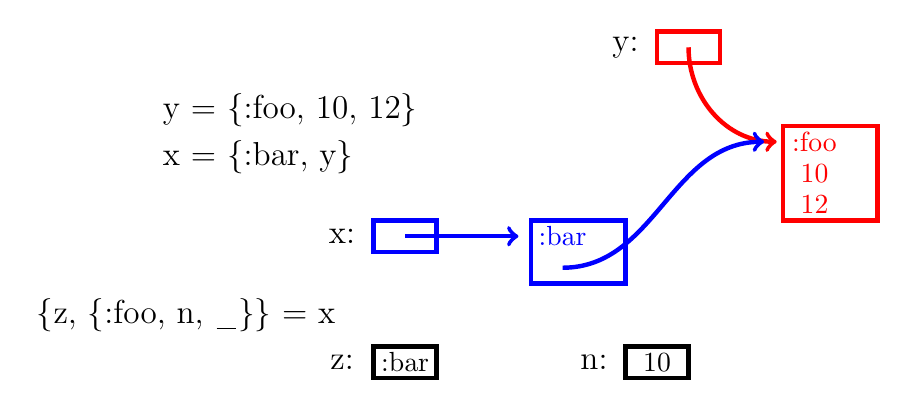
\begin{tikzpicture}[scale=0.4]


\node[anchor=west] at (0,6.5) {{\large y = \{:foo, 10, 12\}}};

\node at (15,8.5) {{\large y:}};
\draw[ultra thick, red] (16,8) rectangle +(2,1);
\draw[ultra thick, red] (20,6)rectangle +(3,-3);
\node[ultra thick, red] at (21,5.5) {:foo};
\node[ultra thick, red] at (21,4.5) {10};
\node[ultra thick, red] at (21,3.5) {12};
\draw[ultra thick, red, ->] (17,8.5) to[out=270,in=180]  (19.8,5.5);

\pause 
\node[anchor=west] at (0,5) {{\large x = \{:bar, y\}}};
\pause 
\node at (6,2.5) {{\large x:}};
\draw [ultra thick, blue] (7,2) rectangle +(2,1);
\draw[ultra thick, blue] (12,3)rectangle +(3,-2);
\node[ultra thick, blue] at (13,2.5) {:bar};
\draw[ultra thick, blue, ->] (13,1.5) to[out=0,in=180]  (19.4,5.5);
\draw[ultra thick, blue, ->] (8,2.5) to[out=0,in=180]  (11.6,2.5);

\pause
\node[anchor=west] at (-4,0) {{\large \{z, \{:foo, n, _\}\}  = x}};


\pause
\draw [ultra thick, black] (7,-2) rectangle +(2,1);
\node at (6,-1.5) {{\large z:}};
\node[ultra thick, black] at (8,-1.5) {:bar};

\draw [ultra thick, black] (15,-2) rectangle +(2,1);
\node at (14,-1.5) {{\large n:}};
\node[ultra thick, black] at (16,-1.5) {10};

\end{tikzpicture}

\end{frame}



\begin{frame}[fragile]{linked list}

  In functional programming languages linked lists are very useful.\pause

  \vspace{20pt}
  \begin{lstlisting}
    []
  \end{lstlisting}
  \vspace{10pt}\pause
  \begin{lstlisting}
    [:one, 2, "three", 4]
  \end{lstlisting}  
  
\end{frame}

\begin{frame}[fragile]{the cons operator}

  Creating a new node:\pause

  \vspace{20pt}
  \begin{lstlisting}
    foo = 1
    rest = [2,3,4,5]
    all = [ foo | rest] 
  \end{lstlisting}
  \vspace{10pt}\pause
  \begin{lstlisting}
    [1,2,3,4,5]
  \end{lstlisting}  
  
\end{frame}

\begin{frame}[fragile]{list patterns}

  \vspace{20pt}
  \begin{lstlisting}
    [a, b, c] = [1,2,3]
  \end{lstlisting}
  \vspace{10pt}\pause
  \begin{lstlisting}
    [a | rest] = [1,2,3]
  \end{lstlisting}  

  \vspace{10pt}\pause
  \begin{lstlisting}
    [a, b | rest] = [1,2,3]
  \end{lstlisting}    

  \vspace{10pt}\pause
  \begin{lstlisting}
    [a | rest] = [1]
  \end{lstlisting}    
\end{frame}


\begin{frame}{exercise}
\begin{itemize}
\pause \item  {\tt [h|t] = [:a,[:b,:c]]}  
\pause \item  {\tt [h1,h2|t] = [:a,:b,:c]} 
\pause \item  {\tt [h1,h2,t] = [:a,:b,:c]} 
\pause \item  {\tt [h1,h2,t] = [:a,:b,:c,:d]} 
\pause \item  {\tt [h1|[h2|t]] = [:a,:b,:c]}
\pause \item  {\tt [h|t] = [:a|:b]}
\end{itemize}
\end{frame}

\begin{frame}{list construction}
\begin{itemize}
\pause \item  {\tt h = :a; t = [:b]; [h|t]}
\pause \item  {\tt h = :a; t = [[:b]]; [h|t]}
\pause \item  {\tt h = [:a,:b]; t = [:c,:d]; [h|t]}
\pause \item  {\tt h = [:a,:b]; t = [:c,:d]; [h,t]}
\pause \item  {\tt h1 = [:a,:b]; h2 = [:c,:d]; t = [:e,:f]; [h1|[h2|t]]}
\pause \item  {\tt h1 = [:a,:b]; h2 = [:c,:d]; t = [:e,:f]; [h1,[h2|t]]}
\pause \item  {\tt h = [:a,:b]; t = :c; [h|t]}
\end{itemize}
\end{frame}


\begin{frame}{cons cells}

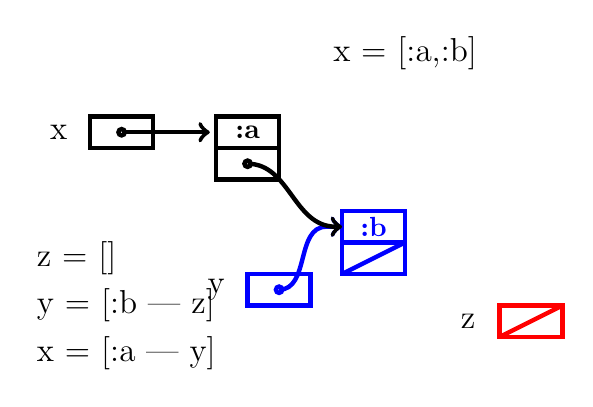
\begin{tikzpicture}[scale=0.4]

\node[anchor=west] at (0,3.5) {{\large z = []}};

\node at (14,1.5) {{\large z}};
\draw [ultra thick, red] (15,1) rectangle +(2,1);
\draw [ultra thick, red] (15,1) -- +(2,1);

\pause 
\node[anchor=west] at (0,2) {{\large y = [:b | z]}};
\pause 
\node at (6,2.5) {{\large y }};
\draw [ultra thick, blue] (7,2) rectangle +(2,1);
\pause 
\draw [ultra thick, blue] (10,4) rectangle +(2,1) node at +(1,0.5) {{\bf :b}};
\draw [ultra thick, blue] (10,3) rectangle +(2,1);
\draw [ultra thick, blue] (10,3) -- +(2,1);
\pause 
\draw [ultra thick, blue] (8, 2.5) circle [radius =0.1];
\draw [ultra thick, blue] (8,2.5)  to [out=0, in=180]  (9.5,4.5);
\draw [ultra thick, blue, ->] (9.5,4.5) -- (10,4.5); 

\pause 
\node[anchor=west] at (0,0.5) {{\large x = [:a | y]}};
\pause 
\node at (1,7.5) {{\large x }};
\draw [ultra thick, black] (2,7) rectangle +(2,1);
\pause 
\draw [ultra thick, black] (6,7) rectangle +(2,1) node at +(1,0.5) {{\bf :a}};
\draw [ultra thick, black] (6,6)  rectangle +(2,1);
\pause 

\draw [ultra thick, black] (7, 6.5) circle [radius =0.1];
\draw [ultra thick, black] (7,6.5)  to [out=0, in=180]  (9.8,4.5);
\draw [ultra thick, black, ->] (9.8, 4.5) -- (10,4.5);
\pause 
\draw [ultra thick, black] (3, 7.5) circle [radius =0.1];
\draw [ultra thick, black, ->] (3,7.5) -- (5.8, 7.5); 
\pause
\node at (12,10) {{\large x = [:a,:b] }};

\end{tikzpicture}

\end{frame}


\begin{frame}[fragile]{Strings}

\begin{verbatim}
text = "This is a string"
\end{verbatim}
  
\vspace{20pt}  \pause
  
\begin{verbatim}
combined = text <> " that we append to this string"
\end{verbatim}

\vspace{20pt}  \pause

\begin{verbatim}
answer = 42
message = "The answer is #{answer}, but what is the question?"
\end{verbatim}

\end{frame}

\begin{frame}[fragile]{Strings and binaries}

\vspace{20pt}  \pause
\begin{verbatim}  
  <<x, y, z , rest::binary>> = "absdefg"
\end{verbatim}  
  
\end{frame}

\begin{frame}[fragile]{Strings and lists of characters}

\vspace{20pt}  \pause  
\begin{verbatim}
  msg = String.to_charlist("abcde")
\end{verbatim}

\vspace{20pt}  \pause
\begin{verbatim}  
  [x,y,z | rest] = msg
\end{verbatim}

\vspace{20pt}  \pause
\begin{verbatim}  
  msg = [?h, ?e, ?l, ?l, ?o]
\end{verbatim}

\vspace{20pt}\pause
 {\em try in teminal:  IEx.configure(inspect: [charlists: :as_lists])}

\end{frame}

\begin{frame}{Summary}

  \pause
  \begin{itemize}
  \item functions : and only functions \pause
  \item modules : one moule one file  \pause
  \item literals : integer, float, boolean, atom \pause
  \item compund :  tuples, lists \pause
  \item strings:  "hello", ?h, ?e, ?l, ?l, ?o, 'hello'
  \end{itemize}

\end{frame}


\end{document}
